\documentclass{article}
\usepackage[utf8]{inputenc}
\usepackage{amsmath}
\usepackage{amssymb}
\usepackage{amsthm}
\usepackage{outlines}
\usepackage{cancel}
\usepackage{comment}
\usepackage{float}
\usepackage[T1]{fontenc}
\usepackage{hyperref}
\usepackage{graphicx}
\usepackage{listings}
\usepackage{multirow}
\usepackage{parcolumns}
\usepackage[table,xcdraw]{xcolor}
\newcommand{\lands}{\:\land\:}                          % "logical and with spaces". Pone el "y" dejando espacio(mediano) a los costados
\newcommand{\comma}{,\,}                                % Pone la coma seguida de un espacio(chiquito)
\newcommand{\tq}{/\,}                                   % "tal que". Pone la barrita del "tal que" seguida de un espacio
\newcommand{\vees}{\:\vee\:}                            % "vee with spaces". Pone el "ó" con espacio a los costados
\newcommand{\eq}{\:=\:}                                 % Pone el igual con espacios(medianos) a los costados
\newcommand{\neqs}{\:\neq\:}                            % Pone el desigual con espacios(medianos) a los costados
\newcommand{\relates}{\mathcal{R}}                      % Pone la R para denotar cuando un elemento se realciona con otro
\newcommand{\enteros}{\mathbb{Z}}                       % Pone la Z de los números enteros
\newcommand{\naturales}{\mathbb{N}}                     % Pone la N de los números naturales
\newcommand{\racionales}{\mathbb{Q}}                    % Pone la Q de los números racionales
\newcommand{\complejos}{\mathbb{C}}                     % Pone la C de los números complejos
\newcommand{\cuerpo}{\mathbb{K}}                        % Pone la K para denotar un cuerpo (los cuerpos son R,Q o C)
\newcommand{\reales}{\mathbb{R}}                        % Pone la R de los números reales
\newcommand{\vabs}[1]{\left\lvert #1 \right\rvert }     % Pone el módulo y recibe como argumento el número
\newcommand{\Rightarrows}{\: \Rightarrow \:}            % Pone la flecha del "entonces" con espacios(medianos) a los costados
\newcommand{\Leftrightarrows}{\: \Leftrightarrow \:}    % Pone la flecha del "si y solo si" con espacios(medianos)
\newcommand{\existsuniq}{\exists !\,}                   % Pone el "existe un único" dejando un espacio(chiquito) para que no quede tan amontonado
\newcommand{\bld}[1]{\textbf{#1}}
\graphicspath{{./Images/}}

\title{Programacion Imperativa}
\author{Nicolás Margenat}
\date{1Q 2021}

\begin{document}
\maketitle
\tableofcontents

\newpage
\section{C basics}
\subsection{\#include}
\begin{itemize}
	\item \#include <\emph{nombreDelArchivo}> . Busca en un Directorio Especial: \emph{/usr/include y derivados}.
	\item \#include "\emph{nombeDelArchivo}" . Busca en el directorio actual de trabajo (en realidad, primero busca en el directorio actual y despues en el especial).
\end{itemize}

\subsection{Palabras Reservadas en C}
Las palabras reservadas en C son: 
\begin{verbatim}
    auto break case char const continue default do double else enum extern float
    for goto if int long register return short signed sizeof static struct switch
    typedef union unsigned void volatile while inline restrict _Bool _Complex _Imaginary
\end{verbatim}

\subsection{Funciones}
\subsubsection*{Pasaje de parametros}
En lenguaje C el pasaje de parametros se realiza siempre por valor (es decir, se pasa una copia de valor derecho).
\subsubsection*{Definicion - Invocacion - Declaracion}
Definicion de Funcion:
\begin{lstlisting}
    tipoDeRetorno /* Si no ponemos nada el compilador asume int */
    nombreFuncion (tipoPar par1, ..., tipoPar parN) /* Lista de parametro formales */
    {
        /* Proposiciones */
    }
\end{lstlisting}
Invocacion de Funcion:
\begin{lstlisting}
    nombreFuncion(par1, ..., parN); /* Lista de parametros actuales */
    nombreFuncion();
\end{lstlisting}
Declaracion - Prototipo:
\begin{lstlisting}
    tipoRetorno nombreFuncion (listaDeParametros);
\end{lstlisting}

\subsection{Complemento a la base}
El primer digito indica el signo y solo puede ser 0 o 1.
\\$CB(P,K)$ representacion polinomica:
\begin{equation*}
    N = (-1) * d_{k-1} * (p^{k-1}) + p^{k-2} * d_{k-2} + ... + p^1 * d_1 + p^0 * d_0
\end{equation*}
Ejemplo: 
\\$CB(2,5): 11011$
\begin{equation*}
    -5 = -1 * (1) * 2^4 + 2^3 * 1 + 2^2 * 0 + 2^1 * 1 + 2^0 * 1
\end{equation*}
Una regla practica para complementar en sistema binario: Invertir todos los digitos del numero y luego sumarle 1.

%-------------------------------------------------------------------%
\newpage
\section{Preprocesador}
\subsection{Tareas del preprocesador}
\begin{itemize}
    \item Eliminacion de comentarios
    \item Inclusion de archivos
    \item Sustitucion de macros
    \item Compilacion condicional
\end{itemize}
El preprocesador NO analiza la sintaxis de C, solo sustituye.
\\!!! Las directivas pueden aparecer en \emph{cualquier lugar de un archivo} y \bld{tienen vigencia a partir de dicha posicion y hasta el final de la unidad de traduccion}.

\subsection{Macros}
\subsubsection*{Macro de sustitucion simple/Defincion de Constantes simbolicas}
\underline{Sintaxis}:
\begin{lstlisting}
    #define IDENTIFICADOR texto de Reemplazo
\end{lstlisting}
\subsubsection*{Constantes simbolicas predefinidas}
\begin{lstlisting}
    __LINE__    Constante decimal con el nro de la linea actual
    __FILE__    String que contiene el nombre del archivo que se esta compilando
    __DATE__    String con la fecha de compilacion
    __TIME__    String con la hora de compilacion
            \end{lstlisting}
\subsubsection*{Macros con Parametros}
\underline{Sintaxis}:
\begin{lstlisting}
    #define IDENTIF(Arg1,...,ArgN) textoReemplazo
\end{lstlisting}
\subsubsection*{Compilacion condicional}
\underline{Sintaxis}:
\begin{lstlisting}
    #ifdef IDENTIFICADOR
        ...
    #else      //Si se quiere usar elseif poner #else #if
        ...
    #endif
\end{lstlisting}
\subsubsection*{Argumentos variables}
\underline{Sintaxis}:
\begin{lstlisting}
    #define name(fixed_args, ...)
\end{lstlisting}
Ejemplo:
\begin{lstlisting}
    #define imprimir(fmt, ...) printf(fmt, __VA_ARGS__)
\end{lstlisting}

\subsection{Operadores con Macros}
\begin{itemize}
    \item \# Unario. Convierte en cadena de texto cada aparicion de un parametro de la macro en el texto de reemplazo.
    \item \#\# Binario. Concatena los componentes lexicos a los cuales se aplica.
\end{itemize}

%-------------------------------------------------------------------%
\newpage
\section{Tipos de Datos}
% Please add the following required packages to your document preamble:
% \usepackage{multirow}
% \usepackage[table,xcdraw]{xcolor}
% If you use beamer only pass "xcolor=table" option, i.e. \documentclass[xcolor=table]{beamer}
\begin{table}[H]
    \begin{tabular}{|l|lll|c|ll|}
    \hline
    \rowcolor[HTML]{C0C0C0} 
                                                      & \multicolumn{1}{l|}{\cellcolor[HTML]{C0C0C0}Tipo de dato}             & \multicolumn{2}{l|}{\cellcolor[HTML]{C0C0C0}Espacio en Memoria} & Tipo Arquitectura                                                                   & \multicolumn{2}{c|}{\cellcolor[HTML]{C0C0C0}Rango}                                                                            \\ \hline
    \rowcolor[HTML]{EBD178} 
    \cellcolor[HTML]{C0C0C0}                          & \multicolumn{1}{c|}{\cellcolor[HTML]{EBD178}}                         & short int                        & 2 bytes                      & \cellcolor[HTML]{EBD178}                                                            & signed                                             & {[}-2\textasciicircum{}31,2\textasciicircum{}31 -1{]}                    \\ \cline{3-4} \cline{6-7} 
    \rowcolor[HTML]{EBD178} 
    \cellcolor[HTML]{C0C0C0}                          & \multicolumn{1}{c|}{\cellcolor[HTML]{EBD178}}                         & int                              & 4 bytes                      & \cellcolor[HTML]{EBD178}                                                            & \cellcolor[HTML]{EBD178}                           & \cellcolor[HTML]{EBD178}                                                 \\ \cline{3-4}
    \rowcolor[HTML]{EBD178} 
    \cellcolor[HTML]{C0C0C0}                          & \multicolumn{1}{c|}{\cellcolor[HTML]{EBD178}}                         & long int                         & 8 bytes                      & \multirow{-3}{*}{\cellcolor[HTML]{EBD178}Arquitectura 4 bytes}                      & \multirow{-2}{*}{\cellcolor[HTML]{EBD178}unsigned} & \multirow{-2}{*}{\cellcolor[HTML]{EBD178}{[}0, 2\textasciicircum{}62{]}} \\ \cline{3-7} 
    \rowcolor[HTML]{EBD178} 
    \cellcolor[HTML]{C0C0C0}                          & \multicolumn{1}{c|}{\cellcolor[HTML]{EBD178}}                         & \multicolumn{2}{l|}{\cellcolor[HTML]{EBD178}}                   & \multicolumn{1}{r|}{\cellcolor[HTML]{EBD178}}                                       & signed                                             & {[}-2\textasciicircum{}15,2\textasciicircum{}15 -1{]}                    \\ \cline{6-7} 
    \rowcolor[HTML]{EBD178} 
    \cellcolor[HTML]{C0C0C0}                          & \multicolumn{1}{c|}{\multirow{-5}{*}{\cellcolor[HTML]{EBD178}int}}    & \multicolumn{2}{l|}{\multirow{-2}{*}{\cellcolor[HTML]{EBD178}}} & \multicolumn{1}{r|}{\multirow{-2}{*}{\cellcolor[HTML]{EBD178}Arquitectura 2 bytes}} & unsigned                                           & {[}0, 2\textasciicircum{}30{]}                                           \\ \cline{2-7} 
    \rowcolor[HTML]{EB6C70} 
    \cellcolor[HTML]{C0C0C0}                          & \multicolumn{1}{l|}{\cellcolor[HTML]{EB6C70}char}                     &                                  & 1byte                        & \cellcolor[HTML]{EB6C70}                                                            & signed                                             & {[}-128, 127{]}                                                          \\ \cline{2-4} \cline{6-7} 
    \rowcolor[HTML]{EB6C70} 
    \cellcolor[HTML]{C0C0C0}                          & \multicolumn{3}{l}{\cellcolor[HTML]{EB6C70}}                                                                                            & \cellcolor[HTML]{EB6C70}                                                            & unsigned                                           & {[}0, 255{]}                                                             \\ \cline{6-7} 
    \rowcolor[HTML]{EB6C70} 
    \multirow{-8}{*}{\cellcolor[HTML]{C0C0C0}Enteros} & \multicolumn{3}{l}{\multirow{-2}{*}{\cellcolor[HTML]{EB6C70}}}                                                                          & \multirow{-3}{*}{\cellcolor[HTML]{EB6C70}Cualquiera}                                & char                                               & {[}??, ??{]}                                                             \\ \hline
    \rowcolor[HTML]{84EBA0} 
    \cellcolor[HTML]{C0C0C0}                          & \multicolumn{1}{l|}{\cellcolor[HTML]{84EBA0}float}                    &                                  & 4 bytes                      & Cualquiera                                                                          & \multicolumn{2}{l|}{\cellcolor[HTML]{84EBA0}}                                                                                 \\ \cline{2-7} 
    \rowcolor[HTML]{50B0B3} 
    \cellcolor[HTML]{C0C0C0}                          & \multicolumn{1}{l|}{\cellcolor[HTML]{50B0B3}}                         & double                           & 8 bytes                      & \cellcolor[HTML]{50B0B3}                                                            & \multicolumn{2}{l|}{\cellcolor[HTML]{50B0B3}}                                                                                 \\ \cline{3-4}
    \rowcolor[HTML]{50B0B3} 
    \multirow{-3}{*}{\cellcolor[HTML]{C0C0C0}Reales}  & \multicolumn{1}{l|}{\multirow{-2}{*}{\cellcolor[HTML]{50B0B3}double}} & long double                      & 16 bytes                             & \multirow{-2}{*}{\cellcolor[HTML]{50B0B3}Cualquiera}                                & \multicolumn{2}{l|}{\multirow{-2}{*}{\cellcolor[HTML]{50B0B3}}}                                                               \\ \hline
    \end{tabular}
    \end{table}
Default:
\begin{itemize}
    \item int = signed int
    \item char = NO TIENE
\end{itemize}
\leavevmode\begin{table}[H]\centering
    \begin{tabular}{|l|l|}
    \hline
    \rowcolor[HTML]{C0C0C0} 
    \multicolumn{2}{|c|}{\cellcolor[HTML]{C0C0C0}\textbf{Abreviaciones del tipo int}} \\ \hline
    \rowcolor[HTML]{EBD178} 
    short int                                 & short                                 \\ \hline
    \rowcolor[HTML]{D4B961} 
    long int                                  & long                                  \\ \hline
    \rowcolor[HTML]{EBD078} 
    unsigned short int                        & unsigned short                        \\ \hline
    \rowcolor[HTML]{F7D872} 
    unsigned long int                         & unsigned long                         \\ \hline
    \end{tabular}
    \end{table}

\subsection{Punteros}
\begin{lstlisting}
    tipoDeDato * nombrePuntero; // Puntero que apunta a una zona donde hay un dato de tipo tipoDeDato
    void * nombrePuntero2; // Puntero generico
\end{lstlisting}
\underline{Apuntes}:
\begin{itemize}
    \item Un puntero a void NO puede ser desreferenciado.
\end{itemize}

%-------------------------------------------------------------------%
\newpage
\section{Reglas de Conversion de Operandos}
\begin{minipage}[c]{.45\textwidth}
    A operador B
\end{minipage}
\begin{itemize}
    \item Si alguno es \emph{long double}, se convierte al otro en \emph{long double}.
    \item Si alguno es \emph{double}, se convierte al otro en \emph{double}.
    \item Si alguno es \emph{float}, se convierte al otro en \emph{float}.
    \item Se convierten los operadores tipo \emph{char} o \emph{short} en \emph{int} o \emph{unsigned int} segun sea necesario.
    \item Si alguno es \emph{unsigned long int}, convertir al otro en \emph{unsigned long int}.
    \item Si uno es \emph{long int} y el otro es \emph{unsigned int}, se convierten a \emph{long int} o \emph{unsigned long int} según sea necesario.
    \item Si alguno es \emph{long int}, convertir al otro en \emph{long int}.
    \item Si alguno es \emph{unsigned int}, convertir al otro en \emph{unsigned int}.
\end{itemize}

%-------------------------------------------------------------------%
\newpage
\section{Constantes}
Las constantes se guardan como \emph{int}(2 o 4 bytes en memoria)
\subsection{Tipos Asumidos}
\begin{table}[H]\centering
    \begin{tabular}{|c|c|l|}
    \hline
    \multicolumn{3}{|c|}{\textbf{Tipos Asumidos}}                                                                                                                                                                                                                \\ \hline
    \rowcolor[HTML]{C0C0C0} 
    \textbf{\begin{tabular}[c]{@{}c@{}}Tipo de\\ Constante\end{tabular}}                                                              & \multicolumn{2}{c|}{\cellcolor[HTML]{C0C0C0}\textbf{\begin{tabular}[c]{@{}c@{}}Tipo Asumido\\ (Creciente)\end{tabular}}} \\ \hline
    \rowcolor[HTML]{EBD178} 
    \cellcolor[HTML]{EBD178}                                                                                                          & int                                                               & 1                                                    \\ \cline{2-3} 
    \rowcolor[HTML]{EBD178} 
    \cellcolor[HTML]{EBD178}                                                                                                          & long                                                              & 2                                                    \\ \cline{2-3} 
    \rowcolor[HTML]{EBD178} 
    \multirow{-3}{*}{\cellcolor[HTML]{EBD178}\textbf{\begin{tabular}[c]{@{}c@{}}Constantes\\ Decimales\end{tabular}}}                 & unsigned long                                                     & 3                                                    \\ \hline
    \rowcolor[HTML]{50B0B3} 
    \cellcolor[HTML]{50B0B3}                                                                                                          & int                                                               & 1                                                    \\ \cline{2-3} 
    \rowcolor[HTML]{50B0B3} 
    \cellcolor[HTML]{50B0B3}                                                                                                          & unsigned int                                                      & 2                                                    \\ \cline{2-3} 
    \rowcolor[HTML]{50B0B3} 
    \cellcolor[HTML]{50B0B3}                                                                                                          & long                                                              & 3                                                    \\ \cline{2-3} 
    \rowcolor[HTML]{50B0B3} 
    \multirow{-4}{*}{\cellcolor[HTML]{50B0B3}\textbf{\begin{tabular}[c]{@{}c@{}}Constantes\\ Octales o\\ Hexadecimales\end{tabular}}} & unsigned long                                                     & 4                                                    \\ \hline
    \end{tabular}
    \end{table}

\subsection{Modificacion de Tipos Asumidos}
Por cuestiones de estilo, ponemos letras mayusculas para determinar el tipo de dato asumido.
\\\bld{Constantes de Tipo int}
\begin{lstlisting}
    135   -----> signed int
    135L  -----> signed long
    135U  -----> unsigned int
    135UL -----> unsigned long
\end{lstlisting}
\bld{Constantes en Punto Flotante}
\begin{lstlisting}
    1.7F  -----> float
    2.1   -----> double
    16.3L -----> long double
\end{lstlisting}

\subsection{Constantes Caracter}
\begin{table}[H]\centering
    \begin{tabular}{|l|l|}
    \hline
    \multicolumn{2}{|c|}{\cellcolor[HTML]{C0C0C0}\textbf{Constantes Caracter}}             \\ \hline
    \textbf{\textbackslash{}a}                & beep                                       \\ \hline
    \textbf{\textbackslash{}b}                & backspace                                  \\ \hline
    \textbf{\textbackslash{}f}                & Comienzo de una nueva pagina               \\ \hline
    \textbf{\textbackslash{}n}                & newline                                    \\ \hline
    \textbf{\textbackslash{}r}                & Retorno de carro                           \\ \hline
    \textbf{\textbackslash{}t}                & tabulador                                  \\ \hline
    \textbf{\textbackslash{}0}                & Caracter nulo (null)                       \\ \hline
    \textbf{\textbackslash{}\textbackslash{}} & Barra invertida                            \\ \hline
    \textbf{\textbackslash{}'}                & Comilla simple                             \\ \hline
    \textbf{\textbackslash{}"}                & Comilla doble                              \\ \hline
    \textbf{\textbackslash{}ooo}              & Caracter cuyo ASCII es el numero octal ooo \\ \hline
    \textbf{\textbackslash{}xhh}              & Caracter cuyo ASCII es el numero hexa hh   \\ \hline
    \end{tabular}
    \end{table}

\subsection{Constantes de enumeracion}
Lista de valores \emph{enteros constantes}
\\\underline{Sinaxis}:
\begin{lstlisting}
    enum nombre { listaDeConstantes };
\end{lstlisting}
Siempre asignar el valor de la primera constante para evitar posibles errores en distintos compiladores.

%-------------------------------------------------------------------%
\newpage
\section{Arreglos}
Los arreglos pueden ser de cualquier de tipo de dato y la cantidad de elementos debe ser un entero.
\\\underline{Sintaxis}:
\begin{lstlisting}
    tipo nombreArreglo[cantidad];
    tipo nombreArreglo[cantidad] = {valor0, valor1, ..., valorCantidad-1};
    tipo nombreArreglo[] = {valor0, valor1, ..., valorCantidad-1};
\end{lstlisting}
\underline{Notas}:
\begin{enumerate}
    \item Al momento de inicializar el arreglo el numero de elementos que va a tener solo puede ser un numero natural.
    \item El primer indice es 0 y el ultimo es cantidad-1.
    \item Si no inicializas todas las variables rellena con 0s.
    \item Solo puedo conocer la cantidad de elementos de un arreglo si esta en el mismo bloque de codigo, y se puede hacer de la siguiente manera:
    \begin{lstlisting}
        sizeof(array) / sizeof(array[0])
    \end{lstlisting}
\end{enumerate}
\subsection{Arreglos bidimensionales}
\underline{Sintaxis de Declaracion}:
\begin{lstlisting}
    tipo matriz[filas][columnas];
    tipo matriz[filas][columnas] = {
    {valor00,valor01, ... ,valor0N},
    {valor10,valor11, ... ,valor1N},
    ...
    {valorN0,valorN1, ... ,valorNN} };
    tipo matriz[][columnas] = {
    {valor00,valor01, ... ,valor0N},
    {valor10,valor11, ... ,valor1N},
    ...
    {valorN0,valorN1, ... ,valorNN} };
\end{lstlisting}
\underline{Sintaxis de Acceso a la componente}:
\begin{lstlisting}
    matriz[i][j]
\end{lstlisting}
\underline{Sintaxis para la Declaracion de un Parametro de tipo arreglo}:
\\IMPRESCINDIBLE INDICAR LA CANTIDAD DE COLUMNAS:
\begin{lstlisting}
    tipo funcion(tipo matriz[][MAXCOL]);
    tipo funcion(tipo matriz[MAXFIL][MAXCOL]);
    tipo funcion(tipo datos[][M1][M2][M3]);
\end{lstlisting}

%-------------------------------------------------------------------%
\newpage
\section{Punteros}
Es una variable que almacena la direccion de otra variable.'
\\\underline{Sintaxis de declaracion}:
\begin{lstlisting}
    tipoApuntado *nombrePuntero;
\end{lstlisting}
\subsubsection*{Equivalencia entre Arreglos y Punteros}
\begin{lstlisting}
     arreglo <==> &arreglo[0]
    *arreglo <==> arreglo[0]
\end{lstlisting}

\subsection{Punteros como paramtros de una funcion}
Cuando una funcion tiene que devolver cierta respuesta, le pasamos la direccion de una zona de memoria
donde dejar dicha respuesta.
\\\underline{Sintaxis de definicion de parametro formal}:
\begin{lstlisting}
    tipo nombreFunc (tipo *nombreParam, ... );
\end{lstlisting}
\underline{Sintaxis de invocacion}:
\begin{lstlisting}
    nombreFunc(&variable);
    nombreFunc(variablePunt);
\end{lstlisting}

\subsection{Operadores de Punteros}
\begin{table}[H]\centering
\begin{tabular}{|c|c|c|}
\hline
\rowcolor[HTML]{C0C0C0} 
\textbf{Operador} & \textbf{Significado}                                                                                                                                                                        & \textbf{Aridad} \\ \hline
\&                & \begin{tabular}[c]{@{}c@{}}Se aplica a un l-value y devuelve la direccoin de\\ memoria donde dicho l-value esta almacenado\end{tabular}                                                     & Unario          \\ \hline
*                 & \begin{tabular}[c]{@{}c@{}}Se aplica a un tipo puntero y devuelve el \\ r-value al cual apunta. Se dice que "desreferencia"\\ al puntero, obteniendo el valor apuntado por el.\end{tabular} & Unario          \\ \hline
\end{tabular}
\end{table}
\underline{Nota}: Un puntero debe ser inicializado antes de ser desreferenciado.
\\\bld{NULL} = constante simbolica (definida en stdio.h) utilizada para indicar
que un puntero apunta a "nada".

\subsection{Operaciones aritmeticas validas}
\begin{lstlisting}
    puntero++; ++puntero; puntero--; --puntero;
    puntero1 - puntero2 //(si puntero2 - puntero1 < 0)
\end{lstlisting}

\begin{table}[H] \centering
\begin{tabular}{|c|}
\hline
\rowcolor[HTML]{C0C0C0} 
\textbf{Operaciones de Asignacion} \\ \hline
puntero1 += numero                \\ \hline
puntero1 -= numero                \\ \hline
puntero1 = puntero2               \\ \hline
\end{tabular}
\end{table}

\begin{table}[H] \centering
\begin{tabular}{|c|}
\hline
\rowcolor[HTML]{C0C0C0} 
\textbf{Operaciones de Comparacion} \\ \hline
puntero1 = = puntero2              \\ \hline
puntero1 != puntero2               \\ \hline
puntero1 \textless{}= puntero2     \\ \hline
puntero1 \textless puntero2        \\ \hline
puntero1 \textgreater{}= puntero2  \\ \hline
puntero1 \textgreater puntero2     \\ \hline
\end{tabular}
\end{table}

%-------------------------------------------------------------------%
\newpage
\section{Strings}
Una constante de tipo string es un arreglo de chars que
no tiene nombre, por lo tanto ella misma representa la
dirección de memoria de la primera componente.
\subsubsection*{¿Dónde se pueden utilizar los strings constantes?}
\begin{enumerate}
    \item Inicializando punteros a char:
    \begin{lstlisting}
        char *texto = "Hola";
    \end{lstlisting}
    \item Asignando punteros a char:
    \begin{lstlisting}
        char *texto;
        texto = "Hola";
    \end{lstlisting}
    \item Como argumento de la funcion:
    \begin{lstlisting}
        printf("Hola");
    \end{lstlisting}
    \item En referencias de punteros a char:
    \begin{lstlisting}
        printf("%s", "Hola" + 2); // Imprime "la"
    \end{lstlisting}
\end{enumerate}

\subsection{Diferencias entre puntero a char, arreglo de chars y string constante}
\begin{center}
    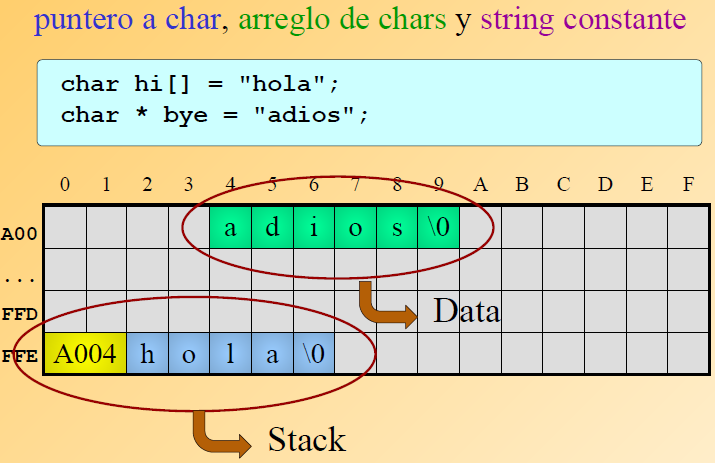
\includegraphics[width=.60\textwidth]{distintosTiposPunteros.PNG}
\end{center}
%-------------------------------------------------------------------%
\newpage
\section{Operadores}
\subsection{Operadores Aritmeticos}
\begin{table}[H]\centering
    \begin{tabular}{c|c|c}
    \hline
    \rowcolor[HTML]{C0C0C0} 
    \multicolumn{1}{|l|}{\cellcolor[HTML]{C0C0C0}Operador} & \multicolumn{1}{|l|}{\cellcolor[HTML]{C0C0C0}Significado}                                                                                                                 & \multicolumn{1}{l|}{\cellcolor[HTML]{C0C0C0}Aridad} \\ \hline
    \multicolumn{1}{|c|}{-}                                & Opuesto                                                                                                                                                                  & \multicolumn{1}{c|}{Unario}                         \\ \hline
    \multicolumn{1}{|c|}{+}                                & Identico valor                                                                                                                                                           & \multicolumn{1}{c|}{Unario}                         \\ \hline
    \multicolumn{1}{|c|}{*}                                & Multiplicación                                                                                                                                                           & \multicolumn{1}{c|}{Binario}                        \\ \hline
    \multicolumn{1}{|c|}{/}                                & Division                                                                                                                                                                 & \multicolumn{1}{c|}{Binario}                        \\ \hline
    \multicolumn{1}{|c|}{+}                                & Adicion                                                                                                                                                                  & \multicolumn{1}{c|}{Binario}                        \\ \hline
    \multicolumn{1}{|c|}{-}                                & Sustraccion                                                                                                                                                              & \multicolumn{1}{c|}{Binario}                        \\ \hline
    \multicolumn{1}{|c|}{\%}                               & Modulo                                                                                                                                                                   & \multicolumn{1}{c|}{Binario}                        \\ \cline{1-1} \cline{3-3} 
    \multicolumn{1}{l|}{}                                  & \multicolumn{1}{l|}{\begin{tabular}[c]{@{}l@{}}- SOLO PARA int\\  - Si uno de los operandos es negativo, el signo\\ del resultado depende de la arquitectura\end{tabular}} & \multicolumn{1}{l}{}                                \\ \cline{2-2}
    \end{tabular}
    \end{table}

\subsection{Operadores Relacionales}
\begin{table}[H]\centering
    \begin{tabular}{ccc}
    \hline
    \rowcolor[HTML]{C0C0C0} 
    \multicolumn{1}{|l|}{\cellcolor[HTML]{C0C0C0}Operador} & \multicolumn{1}{l|}{\cellcolor[HTML]{C0C0C0}Significado} & \multicolumn{1}{l|}{\cellcolor[HTML]{C0C0C0}Aridad} \\ \hline
    \multicolumn{1}{|c|}{\textless{}}                      & \multicolumn{1}{c|}{Menor}                               & \multicolumn{1}{c|}{Binario}                        \\ \hline
    \multicolumn{1}{|c|}{\textless{}=}                     & \multicolumn{1}{c|}{Menor o igual}                       & \multicolumn{1}{c|}{Binario}                        \\ \hline
    \multicolumn{1}{|c|}{\textgreater{}}                   & \multicolumn{1}{c|}{Mayor}                               & \multicolumn{1}{c|}{Binario}                        \\ \hline
    \multicolumn{1}{|c|}{\textgreater{}=}                  & \multicolumn{1}{c|}{Mayor o igual}                       & \multicolumn{1}{c|}{Binario}                        \\ \hline
    \multicolumn{1}{|c|}{==}                               & \multicolumn{1}{c|}{Igual}                               & \multicolumn{1}{c|}{Binario}                        \\ \hline
    \multicolumn{1}{|c|}{!=}                               & \multicolumn{1}{c|}{Distinto}                            & \multicolumn{1}{c|}{Binario}                        \\ \hline
    \multicolumn{1}{l}{}                                   & \multicolumn{1}{l}{}                                     & \multicolumn{1}{l}{}                               
    \end{tabular}
    \end{table}

\subsection{Operadores Logicos}
\begin{table}[H]\centering
    \begin{tabular}{cccl}
    \hline
    \rowcolor[HTML]{C0C0C0} 
    \multicolumn{1}{|c|}{\cellcolor[HTML]{C0C0C0}Operador} & \multicolumn{1}{c|}{\cellcolor[HTML]{C0C0C0}Significado} & \multicolumn{1}{c|}{\cellcolor[HTML]{C0C0C0}Aridad} & \multicolumn{1}{c|}{\cellcolor[HTML]{C0C0C0}Lazy?} \\ \hline
    \multicolumn{1}{|c|}{!}                                & \multicolumn{1}{c|}{Not}                                 & \multicolumn{1}{c|}{Unario}                         & \multicolumn{1}{c|}{NO}                            \\ \hline
    \multicolumn{1}{|c|}{\&\&}                             & \multicolumn{1}{c|}{And}                                 & \multicolumn{1}{c|}{Binario}                        & \multicolumn{1}{c|}{SI}                            \\ \hline
    \multicolumn{1}{|c|}{||}                               & \multicolumn{1}{c|}{Or}                                  & \multicolumn{1}{c|}{Binario}                        & \multicolumn{1}{c|}{SI}                            \\ \hline
    \multicolumn{1}{l}{}                                   & \multicolumn{1}{l}{}                                     & \multicolumn{1}{l}{}                                &                                                   
    \end{tabular}
    \end{table}
Las comparaciones, los operadores lógicos ( \&\&, || , !) devuelven 1 si es verdadero, 0 si es falso.

\subsection{Operadores de Manipulacion de Bits}
SOLO PARA ENTEROS
\begin{table}[H]\centering
    \begin{tabular}{|c|c|c|}
    \hline
    \rowcolor[HTML]{C0C0C0} 
    Operador                     & Significado       & Aridad  \\ \hline
    $\sim$                       & Complemento a 1   & Unario  \\ \hline
    \textless{}\textless{}       & Decalaje a la Izq & Binario \\ \hline
    \textgreater{}\textgreater{} & Decalaje a la Der & Binario \\ \hline
    \&                           & And a nivel bit   & Binario \\ \hline
    |                            & Or a nivel bit    & Binario \\ \hline
    \textasciicircum{}           & Xor a nivel bit   & Binario \\ \hline
    \end{tabular}
    \end{table}

\subsection{Operadores de Incremento y Decremento}
La operacion con estos operandos devuelve un valor del mismo tipo del operando.
\begin{table}[H]\centering
    \begin{tabular}{|c|c|c|}
    \hline
    \rowcolor[HTML]{C0C0C0} 
    Operador & Significado              & Aridad \\ \hline
    ++       & Pre/post incremento en 1 & Unario \\ \hline
    --       & Pre/post incremento en 1 & Unario \\ \hline
    \end{tabular}
    \end{table}
\begin{lstlisting}
    ++variable = Primero modifica la variable y despues la usa
    variable++ = Primero usa la variable y despues la modifica
\end{lstlisting}

\subsection{Operador de Asignación}
\begin{table}[H]\centering
    \begin{tabular}{|c|c|l|}
    \hline
    \rowcolor[HTML]{C0C0C0} 
    Operador & Significado & Aridad  \\ \hline
    =        & Asignación  & Binario \\ \hline
    \end{tabular}
    \end{table}

\subsection{Operador Condicional}
\begin{table}[H]\centering
    \begin{tabular}{|c|l|l|}
    \hline
    \rowcolor[HTML]{C0C0C0} 
    \textbf{Operador}                                                       & \textbf{Significado}                                                                                                                                                & \textbf{Aridad}               \\ \hline
    \textbf{\begin{tabular}[c]{@{}c@{}}oper1?\\ oper2 : oper3\end{tabular}} & \multicolumn{1}{c|}{\begin{tabular}[c]{@{}c@{}}Se evalua oper1, si el mismo\\ es verdadero se evalua solo oper 2,\\ si es falso se evalua solo oper3.\end{tabular}} & \multicolumn{1}{c|}{Ternario} \\ \hline
    \end{tabular}
    \end{table}
Como se lee?:
\begin{lstlisting}
    a = (b > c)? b : c
    "b es mayor que c? Entonces devolveme b, de lo contrario c".
\end{lstlisting}

\subsection{Operador Coma}
\begin{table}[H]\centering
    \begin{tabular}{|c|c|c|}
    \hline
    \rowcolor[HTML]{C0C0C0} 
    {\color[HTML]{000000} \textbf{Operador}} & {\color[HTML]{000000} \textbf{Significado}}                                                                                         & {\color[HTML]{000000} \textbf{Aridad}} \\ \hline
    \textbf{oper1, oper2}                    & \begin{tabular}[c]{@{}c@{}}Se evalua de Izq. a Der.,\\ descartando el valor de oper1 y\\ devolviendo el valor de oper2\end{tabular} & Binario                                \\ \hline
    \end{tabular}
    \end{table}

\subsection{Operador Sizeof}
\begin{table}[H]\centering
    \begin{tabular}{|c|c|c|}
    \hline
    \rowcolor[HTML]{C0C0C0} 
    {\color[HTML]{000000} \textbf{Operador}}                                             & {\color[HTML]{000000} \textbf{Significado}}                                                                                                  & {\color[HTML]{000000} \textbf{Aridad}} \\ \hline
    \textbf{\begin{tabular}[c]{@{}c@{}}sizeof (operando)\\ sizeof operando\end{tabular}} & \begin{tabular}[c]{@{}c@{}}Numero (entero sin signo)\\ de bytes requeridos para\\ almacenar un objeto con\\ el tipo de operando\end{tabular} & Unario                                 \\ \hline
    \end{tabular}
    \end{table}
El operando puede ser un tipo de dato o una expresión. Cuando se trata de una expresión NO la evalua para producir el resultado.

%-------------------------------------------------------------------%
\newpage
\section{Precedencia y Asociatividad de operadores}
\begin{table}[H]\centering
    \begin{tabular}{|c|c|c|}
    \hline
    \multicolumn{3}{|c|}{\textbf{Tabla de Precedencias}}                                                                                                                                                                          \\ \hline
    \rowcolor[HTML]{C0C0C0} 
    \textbf{\begin{tabular}[c]{@{}c@{}}Importancia \\ (Creciente)\end{tabular}} & \textbf{Operadores}                                                                                       & \textbf{Asoc.}                      \\ \hline
    \cellcolor[HTML]{9BA3EB}\textbf{1}                                          & \cellcolor[HTML]{FFFFFF}( )   {[} {]}  .  -\textgreater{}                                                 & \cellcolor[HTML]{EBD178}Izq. a Der. \\ \hline
    \cellcolor[HTML]{9BA3EB}\textbf{2}                                          & \cellcolor[HTML]{FFFFFF}!  $\sim$ ++  --  +  -  (tipo)  sizeof                                            & \cellcolor[HTML]{50B0B3}Der. a Izq. \\ \hline
    \cellcolor[HTML]{9BA3EB}\textbf{3}                                          & \cellcolor[HTML]{FFFFFF}*  /  \%                                                                          & \cellcolor[HTML]{EBD178}Izq. a Der. \\ \hline
    \cellcolor[HTML]{9BA3EB}\textbf{4}                                          & \cellcolor[HTML]{FFFFFF}+  -  (ambos binarios)                                                            & \cellcolor[HTML]{EBD178}Izq. a Der. \\ \hline
    \cellcolor[HTML]{9BA3EB}\textbf{5}                                          & \cellcolor[HTML]{FFFFFF}\textless{}\textless  \textgreater{}\textgreater{}                                & \cellcolor[HTML]{EBD178}Izq. a Der. \\ \hline
    \cellcolor[HTML]{9BA3EB}\textbf{6}                                          & \cellcolor[HTML]{FFFFFF}\textless  \textless{}=  \textgreater  \textgreater{}=                            & \cellcolor[HTML]{EBD178}Izq. a Der. \\ \hline
    \cellcolor[HTML]{9BA3EB}\textbf{7}                                          & \cellcolor[HTML]{FFFFFF}==  !=                                                                            & \cellcolor[HTML]{EBD178}Izq. a Der. \\ \hline
    \cellcolor[HTML]{9BA3EB}\textbf{8}                                          & \cellcolor[HTML]{FFFFFF}\&                                                                                & \cellcolor[HTML]{EBD178}Izq. a Der. \\ \hline
    \cellcolor[HTML]{9BA3EB}\textbf{9}                                          & \cellcolor[HTML]{FFFFFF}\textasciicircum{}                                                                & \cellcolor[HTML]{EBD178}Izq. a Der. \\ \hline
    \cellcolor[HTML]{9BA3EB}\textbf{10}                                         & \cellcolor[HTML]{FFFFFF}|                                                                                 & \cellcolor[HTML]{EBD178}Izq. a Der. \\ \hline
    \cellcolor[HTML]{9BA3EB}\textbf{11}                                         & \&\&                                                                                                      & \cellcolor[HTML]{EBD178}Izq. a Der. \\ \hline
    \cellcolor[HTML]{9BA3EB}\textbf{12}                                         & ||                                                                                                        & \cellcolor[HTML]{EBD178}Izq. a Der. \\ \hline
    \cellcolor[HTML]{9BA3EB}\textbf{13}                                         & ?:                                                                                                        & \cellcolor[HTML]{50B0B3}Der. a Izq. \\ \hline
    \cellcolor[HTML]{9BA3EB}\textbf{14}                                         & =   +=  -=  *=  \%=  \&=  \textasciicircum{}=  |=  \textless{}\textless{}=  \textgreater{}\textgreater{}= & \cellcolor[HTML]{50B0B3}Der. a Izq. \\ \hline
    \end{tabular}
\end{table}
La precedencia y asociatividad de los operadores estan especificadas completamente, 
pero el \emph{orden de evaluacion de las expresiones es indefinida}. 
\\Excepciones: \&\&  ||  ?:  ,

%-------------------------------------------------------------------%
\section{Entrada y salida de datos}
\subsection{putchar}
\underline{Definción}: Escribe el carácter correspondiente al código indicado en la salida estándar.
\\\underline{Sintaxis}: \begin{lstlisting}
    putchar(valorASCII)
\end{lstlisting}

\subsection{printf}
\underline{Definción}: Permite generar salida estándar con formato.
\\\underline{Sintaxis}: \begin{lstlisting}
    printf("Cadena de formato", expr1, expr2, ...)
\end{lstlisting}
\begin{table}[H] \centering
\begin{tabular}{|c|c|l|}
\hline
\rowcolor[HTML]{FFFFFF} 
\multicolumn{3}{|c|}{\cellcolor[HTML]{FFFFFF}\textbf{Indicadores de conversión}}                                                                                                                \\ \hline
\rowcolor[HTML]{C0C0C0} 
\textbf{\begin{tabular}[c]{@{}c@{}}Símbolo\\ (\%)\end{tabular}} & \textbf{Tipo de Dato} & \multicolumn{1}{c|}{\cellcolor[HTML]{C0C0C0}\textbf{Conversión}}                                      \\ \hline
d, i                                                            & int                   & Número entero con signo en base 10                                                                    \\ \hline
o                                                               & int                   & Número octal sin signo ni cero inicial                                                                \\ \hline
x, X                                                            & int                   & Número hexadecimal sin signo                                                                          \\ \hline
u                                                               & int                   & Número entero sin signo en base 10                                                                    \\ \hline
c                                                               & int                   & Carácter simple                                                                                       \\ \hline
s                                                               & char*                 & Cadena de caracteres                                                                                  \\ \hline
f                                                               & double                & Número decimal en punto fijo                                                                          \\ \hline
e, E                                                            & double                & Número decimal en notación exponencial                                                                \\ \hline
g, G                                                            & double                & \begin{tabular}[c]{@{}l@{}}Con exponente menor a -4 la precisión\\ usa \%e, sino usa \%f\end{tabular} \\ \hline
\end{tabular}
\end{table}

\begin{table}[H]\centering
    \begin{tabular}{|c|l|}
    \hline
    \multicolumn{2}{|c|}{\textbf{Modificadores de la conversión}}                                                                                                                                                                                         \\ \hline
    \rowcolor[HTML]{C0C0C0} 
    \textbf{Simbolo}                                                         & \multicolumn{1}{c|}{\cellcolor[HTML]{C0C0C0}\textbf{Conversión}}                                                                                                           \\ \hline
    \textbf{-}                                                               & Alineamiento a la izquierda                                                                                                                                                \\ \hline
    \textbf{0}                                                               & Rellena con ceros                                                                                                                                                          \\ \hline
    \textbf{\begin{tabular}[c]{@{}c@{}}Un número\\ (Ancho)\end{tabular}}     & \begin{tabular}[c]{@{}l@{}}Indica el ancho minimo del campo, completado\\ con blancos a la izq o der segun corresponda\end{tabular}                                        \\ \hline
    \textbf{*}                                                               & El ancho o la precision la toma del argumento                                                                                                                              \\ \hline
    \textbf{.}                                                               & \begin{tabular}[c]{@{}l@{}}Separa la cantidad de digitos de la parte entera\\ de la precicion\end{tabular}                                                                 \\ \hline
    \textbf{+}                                                               & Imprime con signo, incluso un positivo                                                                                                                                     \\ \hline
    \textbf{\begin{tabular}[c]{@{}c@{}}Un número\\ (Precisión)\end{tabular}} & \begin{tabular}[c]{@{}l@{}}floating point = nro. de digitos decimales\\ strings = nro. max de caracteres a imprimir\\ int = nro. minimo de digitos a imprimir\end{tabular} \\ \hline
    \end{tabular}
    \end{table}

\subsection{scanf}
\underline{Sintaxis}:
\begin{lstlisting}
    int scanf(const char * restrict fmt, ...);
\end{lstlisting}

\begin{table}[H] \centering
\begin{tabular}{|c|c|l|}
\hline
\rowcolor[HTML]{FFFFFF} 
\multicolumn{3}{|c|}{\cellcolor[HTML]{FFFFFF}\textbf{Indicadores de conversión}}                                                                                                                \\ \hline
\rowcolor[HTML]{C0C0C0} 
\textbf{\begin{tabular}[c]{@{}c@{}}Símbolo\\ (\%)\end{tabular}} & \textbf{Tipo de Dato} & \multicolumn{1}{c|}{\cellcolor[HTML]{C0C0C0}\textbf{Conversión}}                                      \\ \hline
d                                                            & int                   & Número entero con signo en base 10                                                                    \\ \hline
o                                                               & int                   & Número octal sin signo ni cero inicial                                                                \\ \hline
x                                                            & int                   & Número hexadecimal sin signo                                                                          \\ \hline
u                                                               & int                   & Número entero sin signo en base 10                                                                    \\ \hline
c                                                               & int                   & Carácter simple                                                                                       \\ \hline
s                                                               & char*                 & Cadena de caracteres                                                                                  \\ \hline
f                                                               & double                & Número decimal en punto fijo                                                                          \\ \hline
[...]                                                               & cadenas                & Letras/Nros/Simbolos (es como las regex)                                                                          \\ \hline
[\textasciicircum{}...]                                                               & negar cadenas                & Letras/Nros/Simbolos (es como las regex)                                                                          \\ \hline
\end{tabular}
\end{table}

\underline{Opcionales}: 
\begin{enumerate}
    \item Caracter de supresion \bld{*}
    \item Numero para la amplitud de campo
    \item h, l o L para amplitu del destino
\end{enumerate}


\subsection{Redireccionamiento}
\begin{table}[H]\centering
    \begin{tabular}{|c|c|}
    \hline
    \rowcolor[HTML]{C0C0C0} 
    \textbf{Símbolo}             & \textbf{Funcionamiento}                                                                                                             \\ \hline
    \textless{}                  & programa \textless archivoEntrada                                                                                                   \\ \hline
    \textgreater{}               & \begin{tabular}[c]{@{}c@{}}programa \textgreater archivoSalida\\ (pisa lo que habia en archivoSalida)\end{tabular}                  \\ \hline
    |                            & programa | otroPrograma                                                                                                             \\ \hline
    \textgreater{}\textgreater{} & \begin{tabular}[c]{@{}c@{}}programa \textgreater{}\textgreater archivoSalida\\ (no pisa lo que habia en archivoSalida)\end{tabular} \\ \hline
    \end{tabular}
    \end{table}

%-------------------------------------------------------------------%
\newpage
\section{Heap}
El heap forma parte de la memoria asignada a un
proceso (programa en ejecución) por el sistema
operativo. El mismo se fracciona en forma dinámica en
bloques de distintos tamaños cada vez que un proceso
solicita un bloque mediante la invocación a malloc.

%-------------------------------------------------------------------%
\newpage
\section{Structs}
Colección de datos heterogéneos y sin orden. Sus elementos se identifican con nombres
\\\underline{\bld{Sintaxis de declaracion de un struct}}:
\begin{lstlisting}
    struct nombreRegistro{
        tipo1 nombreCampo1;
        tipo2 nombreCampo2;
        ...
        tipoN nombreCampoN;
    };
\end{lstlisting}
nombreRegistro es un nuevo tipo, NO es una variable. Por lo tanto no reserva espacio hasta
que declaramos una variable de dicho tipo.
\\\\\underline{\bld{Sintaxis de declaracion de una variable de tipo struct}}:
\begin{lstlisting}
   /* ALTERNATIVA 1 */ 
   struct nombreRegistro{
        tipo1 nombreCampo1;
        tipo2 nombreCampo2;
        ...
        tipoN nombreCampoN;
    } nombreVariable;

   /* ALTERNATIVA 2 */ 
   struct nombreRegistro{
        tipo1 nombreCampo1;
        tipo2 nombreCampo2;
        ...
        tipoN nombreCampoN;
    };
    struct nombreRegistro nombreVariable;

   /* ALTERNATIVA 3 */ 
   /* Podemos usar typedef para simplificarnos la vida */
   typedef struct nombreOptativo{
        tipo1 nombreCampo1;
        tipo2 nombreCampo2;
        ...
        tipoN nombreCampoN;
    } nombreTipo;

    struct nombreOptativo unaVariable; // Esta y la de abajo son equivalentes 
    nombreTipo otraVariable;
\end{lstlisting}

\leavevmode\\\underline{\bld{Inicializacion de una variable de tipo struct}}:
\begin{lstlisting}
    typedef struct {
        char aerolinea[30];
        int vuelo;
        char fecha[10];
        char hora[6];
    } tipoPasaje;

    /* ALTERNATIVA 1 */
    tipoPasaje pasaje = {"Flybondi",905,"20240619", "20:30"};
    
    /* ALTERNATIVA 2 */
    pasaje = (tipoPasaje) {
        .aerolinea = "Flybondi",
        .fecha = "20240619",
        .vuelo = 905,
        .hora = "20:30"
    };
\end{lstlisting}

\subsection*{Jerarquia de Campos}
Al anidar estructuras se establecen jerarquías.
Dos campos dentro de la misma jerarquía deben tener diferentes nombres.
Dos campos de diferente jerarquía pueden coincidir en sus nombres.
\begin{center}
    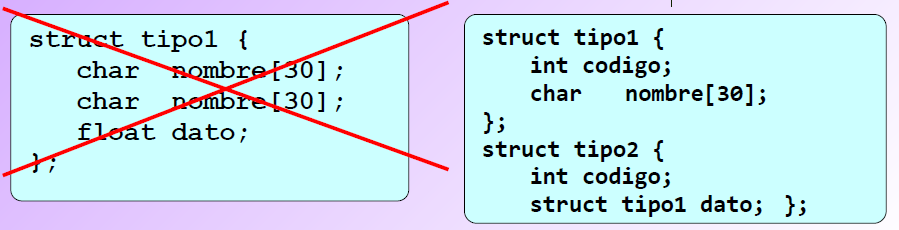
\includegraphics[width=\textwidth]{jerarquiaCampos.PNG}
\end{center}
%-------------------------------------------------------------------%
\newpage
\section{Biblioteca Estandar}
\subsection{stdio.h}
\emph{Standard Input/Output Library}
\begin{lstlisting}
    int getchar(void);
    int putchar(int c);
    int ungetc(int c, FILE *stream);   // Devuelve un caracter al buffer
    int printf(const char *fmt, ...);
    void clearerr(FILE *stream);
    int feof(FILE *stream);            // Devuelve 1 si era EOF
    int ferror(FILE *stream);          // Devuelve 1 si era ERROR
    void perror(const char *s);        // Var global para comunicar mensajes de error
\end{lstlisting}
\underline{Nota}: Hacer 2 ungetc seguidos NO es seguro.

\subsection{stdlib.h}
\emph{Standard System Library}
\begin{lstlisting}
    int abs(int num);       // Devuelve el valor absoluto
    long labs(long num);    // Idem pero con un long int
    int rand(void);         // Devuelve un numero pseudo-aleatorio entre [0, RAND_MAX]
    int srand(unsigned int seed);   // srand se comunica con la funcion rand y empieza con la sucesion desde otro punto. 
    typedef unsigned int size_t;
    void * malloc(size_t size); // Devuelve el puntero a una zona de memoria que yo reserve
    void * calloc(size_t nobj, size_t size); // Idem malloc pero inicializa en 0 la zona
    void * realloc(void * p, size_t size);
    void free(void * p); // Libera la zona de memoria
\end{lstlisting}
\underline{Apuntes}: 
\begin{enumerate}
    \item \emph{rand()} tiene la secuencia armada, entonces siempre te devuelve los mismos valores pq estan ya definidos.
    \item \emph{srand()} se comunica con la funcion \emph{rand()} y empieza con la sucesion desde otro punto. 
    \item \emph{void srand(time(NULL))} para que sea aleatorio \emph{rand()}. 
    \item Nunca poner \emph{void srand(time(NULL))} adentro de loops, sino se va a generar siempre la misma secuencia (porque toma milisegundos).
    \item Por cada malloc() tiene que haber un free().
\end{enumerate}

\subsection{ctype.h}
\emph{Character Type Library}
\\Retornan 0 (verdadero) o un valor distinto de 0 (falso)
\begin{lstlisting}
    int islower(int c);
    int isupper(int c);
    int isalpha(int c);     // Es letra
    int isdigit(int c);
    int isxdigit(int c);    // Es digito hexa
    int isalnum(int c);     // Es letra o digito
    int isprint(int c);
    int ispunct(int c);
    int isspace(int c);
    int iscntrl(int c);
    int isgraph(int c);
    int toupper(int c);
    int tolower(int c);
\end{lstlisting}
\underline{Nota}: Recordar que UNA FUNCION NO MODIFICA EL VALOR DE LA VARIABLE QUE LE PASAS COMO PARAMETRO

\subsection{math.h}
\emph{Math Library}
\begin{lstlisting}
    double fabs(double x);      // Valor absoluto
    double floor(double x);     // Mayor de los enteros menores a x
    double ceil(double x);      // Menor de lo enteros mayores a x
    double fmod(double x,double y);
    double sqrt(double x);      // Si le pasas un valor invalido se va de rango
    double pow(double x,double y);
    double exp(double x);       // e^x
    double log(double x);
    double log10(double x);
    double sin(double angulo);  /*
    double cos(double angulo);  ** Usando radianes
    double tan(double angulo);  */
\end{lstlisting}
\underline{Notas}: Esta biblioteca no se linkedita automaticamente, hay que agregar -lm cuando se compila el codigo.

\subsection{errno.h}
Tiene definidas dos constantes
\begin{lstlisting}
    EDOM = error en el dominio de la funcion
    ERANGE = error en el rango, osea fuera de rango
\end{lstlisting}
\underline{Notas}: Conviene siempre inicializarla en 0 por ser una variable global.

\newpage\subsection{string.h}
String Library
\begin{table}[H] \centering
\begin{tabular}{|l|l|}
\hline
\rowcolor[HTML]{C0C0C0} 
\multicolumn{1}{|c|}{\cellcolor[HTML]{C0C0C0}\textbf{Funcion}} & \multicolumn{1}{c|}{\cellcolor[HTML]{C0C0C0}\textbf{Significado}}                                                                                                          \\ \hline
unsigned int strlen(const char *s)                             & String length                                                                                                                                                              \\ \hline
char *strcpy(char *d, const char*f)                            & Copies the string pointed to, by f to d.                                                                                                                                   \\ \hline
char *strncpy(char *d, const char *f, int n)                   & Copies up to n characters from the string pointed to, \\by f to d.                                                                                                           \\ \hline
char *strcat(char *d, const char*f)                            & \begin{tabular}[c]{@{}l@{}}Appends the string pointed to, \\by f to the end of the string pointed to by d.\end{tabular}                                                    \\ \hline
char *strncat(char *d, const char *f, int n)                   & \begin{tabular}[c]{@{}l@{}}Appends the string pointed to, by f to the \\ end of the string pointed to\\, by d up to n characters long.\end{tabular}                          \\ \hline
int strcmp(const char *d, const char *f)                       & Compares the string pointed to, by str1 to the string \\pointed to by str2.                                                                                                  \\ \hline
int strncmp(const char *d, const char *f, int n)               & Compares at most the first n bytes of str1 and str2.                                                                                                                       \\ \hline
char *strchr(const char *s, char c)                            & \begin{tabular}[c]{@{}l@{}}Searches for the first occurrence of the character\\ c (an unsigned char) in the string pointed to, \\by the argument s.\end{tabular}             \\ \hline
char *strrchr(const char *s, char c)                           & \begin{tabular}[c]{@{}l@{}}Searches for the last occurrence of the \\character c (an unsigned char) in the string pointed to\\ by the argument s.\end{tabular}               \\ \hline
char *strpbrk(const char *s, const char *set)                  & Finds the first character in the string s that matches \\any character specified in set.                                                                                     \\ \hline
char *strstr(const char *d, const char *f)                     & \begin{tabular}[c]{@{}l@{}}Finds the first occurrence of the entire string f\\  (not including the terminating null character) \\which appears in the string d.\end{tabular} \\ \hline
\end{tabular}
\end{table}

\subsection{strings.h}
\begin{lstlisting}
    int strcasecmp(const char *, const char *);
    int strncasecmp(const char *, const char *, size_t); 
\end{lstlisting}
%-------------------------------------------------------------------%
\newpage
\section{Modificadores de Variables}
\underline{Nota}: Las variables globales SIEMPRE se inicializan en 0.
\subsection{static}
Estas variables se crean afuera del stack.
\subsubsection*{Definidas fuera de una funcion}
Similar a la aplicación sobre funciones, la variable es visible solo dentro del módulo donde está definida e invisible al resto de los módulos.
\\\emph{Ejemplo de Invocacion}:
\begin{lstlisting}
    static int a;
\end{lstlisting}
\subsubsection*{Definidas dentro de una funcion}
La variable existe durante toda la ejecución sin perder su valor entre invocación e invocación.
\\\emph{Ejemplo de Invocacion}:
\begin{lstlisting}
    int
    funcion(int valor)
    {
        static int acum = 0;
        acum + = valor;
        return acum;
    }
\end{lstlisting}

\subsection{extern}
Se usa para utilizar una variable global. 
Es para avisarle al compilador que la vas a usar, si esta en el mismo archivo no hace falta.
\subsubsection*{Definidas/Declaradas fuera de una funcion}
Es una variable visible desde todos los archivos que componen el programa.
\\\emph{Ejemplo Invocacion}:
\begin{lstlisting}
    extern int a;
\end{lstlisting}
\subsubsection*{Declarada dentro de funciones}
Es una variable definida en otra zona y referenciada desde la función donde se la declara.

\subsection{const}
Se utiliza para definicr una constante con el espacio de una variable (por ejemplo para definir una constate short).
%-------------------------------------------------------------------%
\newpage
\section{Reglas de estilo}
\subsection{Nombres de Archivos}
\begin{enumerate}
    \item Los nombres de archivos deben comenzar con una letra, continuando con letras (minúsculas) o números.
    \item No utilizar más de 8 caracteres para la parte prefija.
    \item Sufijo .c para los archivos con código fuente en lenguaje C.
    \item Sufijo .h para los archivos de encabezado.
    \item Es conveniente el uso del archivo nombrado README como resumen del contenido que se encuentra en cada directorio.
\end{enumerate}

\subsection{Orden de las Secciones en un Archivo Fuente}
\begin{enumerate}
    \item Prólogo que indique una descripción del propósito del contenido. Debe ademas contener autor, version, referencias.
    \item Inclusión de encabezamientos.
    \item Definición de constantes simbólicas, macros, typedef y enumerativos, que se apliquen a todo el archivo.
    \item Funciones que conforman el programa.
\end{enumerate}

\subsection{Comentarios}
\begin{enumerate}
    \item Los comentarios deben explicar qué se está haciendo y no cómo se lo está haciendo. 
    Solo resulta útil explicar por qué se implementó de determinada forma un fragmento de código, cuando se analizaron varias alternativas y solo la actual resultó aceptable.
    \item Los comentarios deben explicar el significado de los parámetros y las supuestas restricciones de una función.
    \item Los comentarios dentro de las funciones deben estar indentados de la misma forma que el resto del código en donde se encuentran, pudiendo escribirlos en una sola línea.
    Si son muy cortos pueden colocarse al costado del código.
    \item Cuando un comentario se refiere a un bloque debe tener alguno de los siguientes formatos:
    \\\begin{minipage}{.45\textwidth}
    \begin{lstlisting}
/*
* Comentario
* de Bloque
*/
    \end{lstlisting}
    \end{minipage}\hfill
    \begin{minipage}{.45\textwidth}
    \begin{lstlisting}
/*
** Comentario
** de Bloque
*/
    \end{lstlisting}
    \end{minipage}
\end{enumerate}

\subsection{Constantes de Enumeración}
\begin{enumerate}
    \item No conviene tener valores consecutivos con "baches" internos.
    \item Si se usa un enumerativo, conviene que la primera constante sea un valor distinto de cero o sea un valor que indique un caso especial de la lista.
    \item Las constantes enumerativas deben empezar con mayúscula o bien estar todas en mayúsculas.
\end{enumerate}

\subsection{Constantes Simbólicas}
\begin{enumerate}
    \item Los identificadores para las constantes simbólicas deben estar formados por letras mayúsculas.
\end{enumerate}

\subsection{Identificadores}
\begin{enumerate}
    \item Los identificadores no deben tener underscore ni al comienzo ni al final.
    \item Evitar tener identificadores que sólo difieran en una letra, por ser mayúscula en uno y minúscula en otro.
    \item Evitar identificadores que se parezcan mucho entre sí.
    \item Evitar usar la l (letra ele) y el 1 (uno).
    \item Evitar usar nombres de la biblioteca estándar.
\end{enumerate}

\subsection{Proposiciones Simples y Bloques}
\begin{enumerate}
    \item Debe haber sólo una proposición por línea, a menos que las proposiciones estén altamente relacionadas (Ej: break).
    \item Aunque el lenguaje permite resumir varias acciones en una sola expresión, lo que se debe priorizar es la claridad y la mantenibilidad del código.
    Por ejemplo:
    \begin{lstlisting}
        a = b + c;
        d = a + e;
    \end{lstlisting}
    En lugar de:
    \begin{lstlisting}
        d = (a = b + c) + e;
    \end{lstlisting}
    \item Las llaves de un bloque deben estar siempre en una línea separada, y cada proposición del mismo debe estar en una línea aparte, e indentada respecto de las llaves.
\end{enumerate}

\subsection{Proposiciones de Decisión}
\begin{enumerate}
    \item Para consultar variables "booleanas" no es necesario indicar la igualdad.
    Por ejemplo:
    \begin{lstlisting}
        if (esPar != 0)  if(esPar)
    \end{lstlisting}
    \item Hay casos en los que se puede prescindir de la proposición if-else para asignarle a una variable un resultado booleano.
    \item Para proposiciones excluyentes, usar if excluyentes. Por ejemplo:
    \begin{lstlisting}
        if (sueldo < 300)
            printf("Sueldo inicial\n");
        else if (sueldo < 900)
            printf("Sueldo medio\n");
        else
            printf("Sueldo aceptable\n");
    \end{lstlisting}
    \item Cuando se opera con números reales hay que utilizar un rango de tolerancia para analizar igualdad o desigualdad.
\end{enumerate}

\subsection{Espacios y Tabulaciones}
\begin{enumerate}
    \item Usar blancos verticales y horizontales en forma generosa.
    \item La indentación y el espaciado deben reflejar la estructura del bloque del
código.
    \item Una cadena de caracteres larga conteniendo operadores booleanos debe dividirse en líneas separadas, cortando antes de un operador booleano:
    \begin{lstlisting}
        if (a == 5 && total < tope && tope <= MAX)
    \end{lstlisting}
    La forma correcta es:
    \begin{lstlisting}
        if ( a == 5 && total < tope
            && tope <= MAX )
    \end{lstlisting}
\end{enumerate}

\subsection{Funciones}
\begin{enumerate}
    \item Cada funcion debe realizar una única tarea: su nombre debe ser significativo y surgir naturalmente. 
    Si es dificil elegirle un nombre es porque no llega a hacer nada o hace demasiadas cosas.
    \item Cada prototipo de funcion debe ser precedido por un prologo (comentario) que indique que hace y como usarla.
    \item Utilizar programacion defensiva, o sea nunca presuponer que algo jamas va a ocurrir.
    \item Someter cada funcion a pruebas de software: caja blanca y caja negra.
\end{enumerate}

\subsection{Macros}
\begin{enumerate}
    \item Nombres de macros en mayusculas.
    \item Todas las ocurrencias de argumentos entre parentesis.
    \item Si hay operaciones matematicas, encerrar el texto de la macro entre parentesis.
\end{enumerate}

\subsection{Arreglos}
\begin{enumerate}
    \item Para conocer la cantidad de elementos del arreglo (siempre que el arreglo este dentro del bloque donde se 
    lo define) usar:
    \begin{lstlisting}
        sizeof(nombreArray) / sizeof(nombreArray[0])
    \end{lstlisting}
\end{enumerate}

%-------------------------------------------------------------------%
\newpage
\section{Algoritmos}
\subsection*{Bubble Sort}
Comparamos items consecutivos, si estan fuera de lugar los swappeamos.
Al final dell arreglo hay una particion de elementos ordenados, ya que 
el numero mas grande (de cada iteracion) va a "bubblear" hasta el final del arreglo con cada iteracion.
\\\underline{Pseudocodigo}:
\begin{lstlisting}
    for i from 1 to N
        for j from to N -1 
            if a[j] > a[j + 1]
                swap(a[j], a[j + 1])
\end{lstlisting}
\underline{Complejidad}: $O(n^2)$

\subsection*{Selection Sort}
En cada iteracion seleccionamos el item mas chiquito de la particion no ordenada y lo
movemos a la parte ordenada.
\\\underline{Pseudocodigo}:
\begin{lstlisting}
    for(j = 0; j < n-1; j++)
    {
        int iMin = j;
        for(i = j + 1; i < n; i++)
            if(a[i] < a[iMin])
                iMin = i;
        if(iMin != j)
            swap(a[j], a[iMin]);
    }
\end{lstlisting}
\underline{Complejidad}: $O(n^2)$

\subsection*{Algoritmo de Euclides}
Es para encontrar el Maximo Comun Divisor entre dos numeros.
\\\underline{Pseudocodigo}:
\begin{lstlisting}
    aux = num1
    while(aux != 0)
    {
        num1 = num2;
        num2 = aux;
        aux = num1 % num2;
    }

    return num2;
\end{lstlisting}

\end{document}